%!TEX root = ../thesis_a4.tex

\chapter{\titlecap{Automatic \glsentrytext{raga} Recognition}}
\label{chap:raga_recognition}


\section{Introduction}
\label{sec:raga_rec_intro}

In this chapter we address the task of automatically recognizing \glspl{raga} in audio recordings of \gls{iam}. We describe two novel approaches for \gls{raga} recognition that jointly capture the tonal and the temporal aspects of melody. The contents of this chapter are largely based on our published work in~\cite{gulatiphrase_2016} and in~\cite{gulati_tdms_2016}.

As mentioned before, \gls{raga} is a core musical concept used in compositions, performances, music organization, and pedagogy of \gls{iam}. Even beyond the art music, numerous compositions in Indian folk and film music are also based on \glspl{raga}~\citep{ganti2013bollywood}. \Gls{raga} of the musical piece is the most desired melodic description of a recorded performance of \gls{iam} by listeners. Despite its significance, there exists a large volume of audio content whose \gls{raga} is incorrectly labeled or, simply, unlabeled. A computational approach to \gls{raga} recognition will allow us to automatically annotate large collections of audio music recordings. It will enable \gls{raga}-based music retrieval in large audio archives, semantically-meaningful music discovery and musicologically-informed navigation. Furthermore, a deeper understanding of the \gls{raga} framework from a computational perspective will pave the way for building applications for music pedagogy in \gls{iam}. 

\Gls{raga} recognition is the most studied research topic in \gls{mir} of \gls{iam}. There exist a considerable number of approaches utilizing different characteristic aspects of \glspl{raga} such as \gls{svara} set, \gls{svara} salience and \gls{arohana}-\gls{avrohana}. A critical in-depth review of the existing approaches for \gls{raga} recognition is presented in \secref{sec:sota_raga_recognition}, wherein we identify several shortcomings in these approaches and possible venues for scientific contribution to take this task to the next level. Here we provide a short summary of that: 

\begin{itemize}
	\item Around half the number of the existing approaches for \gls{raga} recognition do not utilize the temporal aspects of melody at all (\tabref{tab:raga_recognition_methods_melodic_characteristics}), which are crucial in characterizing \glspl{raga}. Approaches that do utilize the temporal aspects, invariably consider a discrete representation of melody in the analysis . Thus, they fall short of capturing the characteristics of the continuous melodic transitions across the \glspl{svara}, which is a relevant information for \gls{raga} recognition. Therefore, approaches that can work with a continuous melody representation and still can capture effectively the temporal aspects of melody are worth exploring for this task.
	
	\item The musical complexity in recognizing \glspl{raga} depends on both the number and the specific set of \glspl{raga} to be differentiated. A large number of the existing approaches for this task are evaluated using different datasets, which typically comprise a small number of \glspl{raga} with only a handful of recordings per \gls{raga}. Therefore, a reliable assessment and comparison of the existing approaches becomes a challenging task. Thus, a sizable representative dataset of Hindustani and Carnatic music that can be openly shared and used by the community will be instrumental in systematically improving the state-of-the-art in \gls{raga} recognition.
	
	\item A comparative  evaluation of the existing methods is missing in the literature. Most of the studies only evaluate their proposed method and do not perform any comparison with the existing studies. A comprehensive comparison of different approaches on the same dataset and under the same experimental setup is needed in order to identifying the strengths and weaknesses of these methods.
	
\end{itemize}

%\begin{figure}
%	\begin{center}
%		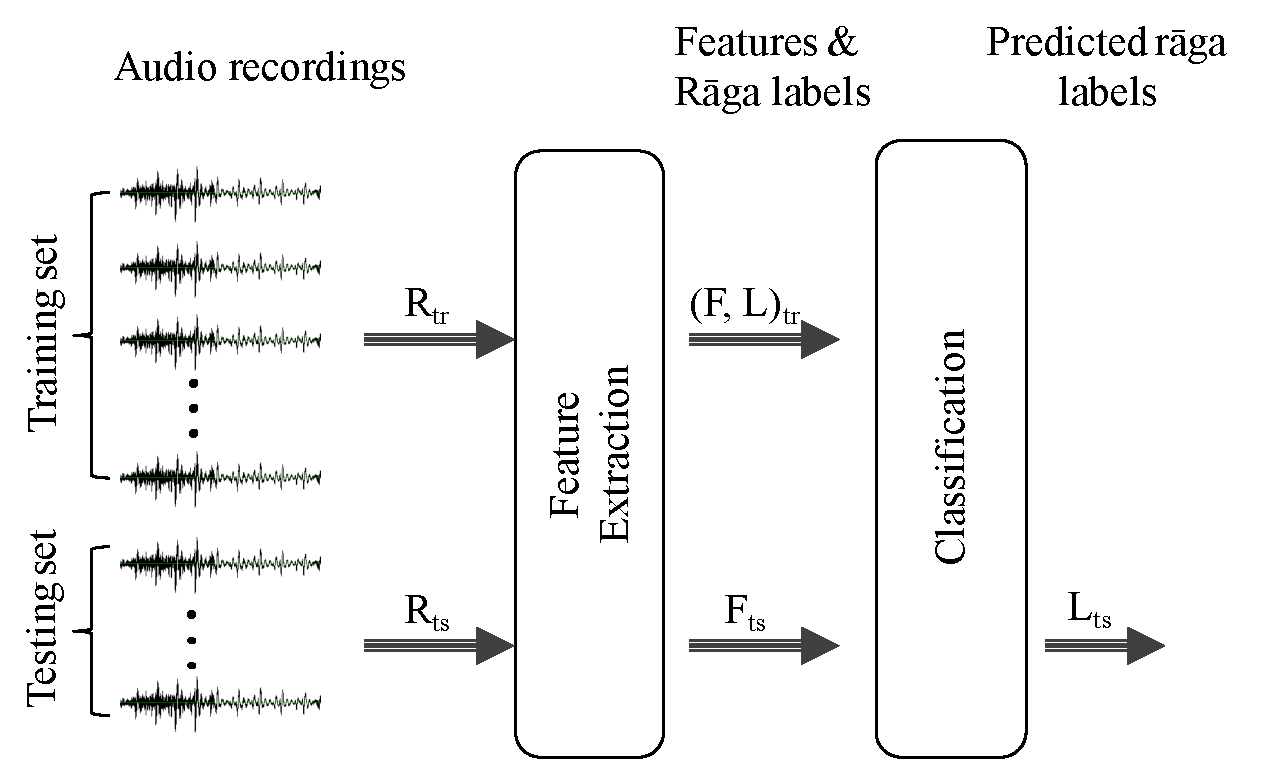
\includegraphics[width=\figSizeEightyFive]{ch07_ragaRecognition/figures/bd_overall_raga_recognition.pdf}
%	\end{center}
%	\caption{Overall block diagram for automatic \gls{raga} recognition.}
%	\label{fig:bd_raga_recognition}
%\end{figure}

In this section we describe two novel methods for \gls{raga} recognition \acrshort{ragarecVSM} and \acrshort{ragarecTDMS} that overcome a number of shortcomings in the existing approaches as enumerated above and in our literature review (\secref{sec:sota_raga_recognition}). In addition, we compile and curate sizable datasets of Hindustani and Carnatic music for evaluating our methods. To the best of our knowledge these are the largest datasets every used for this task. Furthermore, we also make these datasets publicly available online (\appref{app:resources}), which addresses another important issue mentioned above. We now proceed to describe our methods in detail. 

%A general block diagram of \acrshort{ragarecVSM} and \acrshort{ragarecTDMS} is shown in Figure~\ref{fig:bd_raga_recognition}. There are two main processing blocks; feature extraction and classification. Given sets of audio recordings for training ($\mathrm{\corpus}_\mathrm{tr}$) and testing ($\mathrm{\corpus}_\mathrm{ts}$) we first extract features ($\mathrm{F}_\mathrm{tr}$ and $\mathrm{F}_\mathrm{ts}$) for every audio recording in both the sets. Subsequently features of the training set $\mathrm{F}_\mathrm{tr}$ along with the \gls{raga} labels $\mathrm{L}_\mathrm{tr}$ are used to train a classifier to build a classification model. Using this model we then predict the \gls{raga} labels for the testing set $\mathrm{L}_\mathrm{ts}$. \acrshort{ragarecVSM} and \acrshort{ragarecTDMS} differ both in terms of the extracted features and the classification strategy. Both these methods are described at length in the subsequent sections.



\section{\titlecap{Pattern-based \glsentrytext{raga} Recognition}}
\label{sec:pattern_based_raga_recognition}

In this section we describe our pattern-based approach (\acrshort{ragarecVSM}) to \gls{raga} recognition. \acrshort{ragarecVSM} utilizes melodic patterns automatically discovered from audio recordings using our approach described in \chapref{chap:melodic_pattern_processing}, and employs vector space modeling concept to build a \gls{raga} model from these melodic patterns. This section is based on our published work presented in~\cite{gulatiphrase_2016}.

As mentioned before, every \gls{raga} has a set of characteristic melodic patterns that capture the essence of the \gls{raga}. These melodic patterns are one of the most prominent cues for \gls{raga} identification, used by a performer, as well as by a listener (\secref{sec:melody_in_iam}). They act as a building block to construct melodies both in composition and improvisation. However, despite the importance of melodic patterns in characterizing \glspl{raga}, they are not fully exploited by the computational methods for \gls{raga} recognition.  There exist only a handful of methods that utilize melodic patterns for this task (\secref{sec:sota_raga_recognition}). These methods work with a discrete representation of melody and pre-defined dictionaries of melodic patterns, which severely limits the potential of a pattern-based approach for \gls{raga} recognition. To the best of our knowledge there exists only one method that uses automatically discovered melodic patterns for this task~\citep{shrey_ISMIR_2015}. Although, the melodic patterns are extracted from specific short duration regions (Pallavi lines) of recordings in Carnatic music, and therefore, the scalability of this method on large audio collections is questionable. Furthermore, the authors address the task of \gls{raga} verification, which is less challenging compared to \gls{raga} recognition. A detailed discussion on the existing methods and their shortcomings is provided in \secref{sec:sota_raga_recognition}.

Before formally describing our method, we first present the intuition and motivation behind the approach. A number of similarities can be seen between a \gls{raga} rendition and a textual description of a topic. Like an author describes a topic by using different words relevant to the topic, an artist renders a \gls{raga} by using appropriate melodic phrases that suit the context. There are words that are quite specific to a topic, which are analogous to the characteristic melodic phrases of a \gls{raga}. Stop words, which are not specific to any topic or to a document can be seen as generic \gls{gamaka} type melodic patterns, which are not specific to a \gls{raga} or to a recording (\secref{sec:recurring_melodic_patterns_iam}). Words that are specific to a document are analogous to composition specific patterns. This analogy drives our method and motivates us to employ concepts of \gls{vsm} to perform \gls{raga} recognition using melodic patterns. We now proceed to describe \acrshort{ragarecVSM} in detail.

 %As shown in~\figref{fig:bd_raga_recognition} there are two main processing blocks; feature extraction and classification. In the first block we extract TFIDF-based features, wherein we consider automatically discovered melodic patterns as different `terms' (\secref{sec:vsm_feature_extraction}). Based on these features, in the second block we train a classifier to build a model for each \gls{raga}. 

\COMMENT{if time permits write pros and cons of a phrase based approach?}

%Merits and shortcomings of this method are summarized below:
%\begin{itemize}
%	\item Human interpretation of the intermediate output, usability of intermediate outputs, exploiting the most characteristic aspect of a raga. Utilize both the tonal and the pitch information. Exploit characteristic movements between the svaras as well as sequence of svaras
%	\item No need for analyzing whole melody, if patterns are identified in chunks raga can be identified.
%	\item Musically meaningful relatinos between recordings can be established.
%\end{itemize}
%
%Cons
%\begin{itemize}
%	\item Prone to octave errors, not statistical, spurts of error can deprove the performance enormously
%	\item Extraction of characteristic melodic patterns is still a challenging process. Limited by that performance
%	\item Affected a lot by the improvisational aspects
%	\item Computationally challenging. 
%	\item Does not exploit global melodic characteristics.
%\end{itemize}
%

\begin{figure}
	\begin{center}
		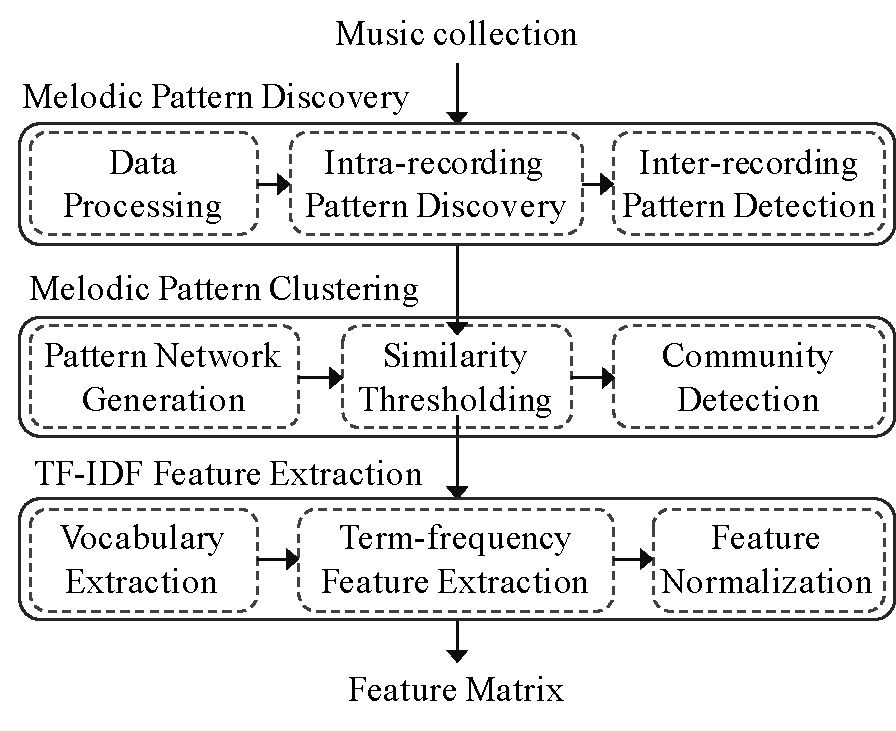
\includegraphics[width=\figSizeSeventy]{ch07_ragaRecognition/figures/bd_phasebased_raga_recognition.pdf}
	\end{center}
	\caption{Block diagram of the proposed phrase-based approach to \gls{raga} recognition.}
	\label{fig:bd_phasebased_raga_recognition}
\end{figure}


\subsection{Vector Space Modeling of Melodic Patterns}
\label{sec:vsm_feature_extraction}

The block diagram of \acrshort{ragarecVSM} is shown in Figure~\ref{fig:bd_phasebased_raga_recognition}. There are three main processing blocks; melodic pattern discovery, pattern clustering and \gls{tfidf}-based feature extraction. Below we describe each of these blocks in detail. 

\subsubsection{Melodic Pattern Discovery}
\label{sec:vsm_feature_extraction_pattern_discovery}

In this block we extract repeating melodic patterns from the collection of audio recordings. For this, we employ the pattern discovery method described in~\secref{sec:patterns_melodic_pattern_discovery}. There are three main processing modules in our pattern discovery method; data-processing, intra-recording pattern discovery and inter-recording pattern search,  which are already described at length in~\secref{sec:patterns_discovery_method}. We use the same set of parameter settings as mentioned in their description. 

\TODO{Provide the params of the latest setting used to report results}

Note that the output of the pattern discovery method contains different types of repeated melodic patterns with their varied degree of musical relevance (\secref{sec:patterns_characterization_of_melodic_patterns}). In this step we do not filter any melodic pattern based on their relevance with respect to \glspl{raga}. A soft selection of the relevant melodic patterns is implicitly done in our methodology described in the subsequent sections.


\subsubsection{Melodic Pattern Clustering}
\label{sec:vsm_feature_extraction_pattern_clustering}

In order to effectively utilize the discovered melodic patterns for \gls{raga} recognition, it is important to cluster together all the patterns that are different occurrences of the same underlying melodic phrase. For this, we propose to perform a network analysis, wherein the clustering is performed using a non-overlapping community detection method. The network analysis and clustering process used here is the same as described in~\secref{pattern_characterization}, but with a different end goal of characterizing melodic patterns. For the sake of completeness we here provide a brief description of the process we follow.

We start by building an undirected network $\netUndirWght$ using the discovered patterns as the nodes of the network. We connect any two nodes only if the distance between them is below a similarity threshold $\simThsld$. Noticeably, the distance between two melodic patterns is computed using the same measure as used in the intra-recording pattern discovery block~(\secref{sec:intraRecordingPatternDiscovery}). The weight of the edge, when it exists, is set to 1, and all non-connected nodes are removed from the network.

\begin{figure}
	\begin{center}
		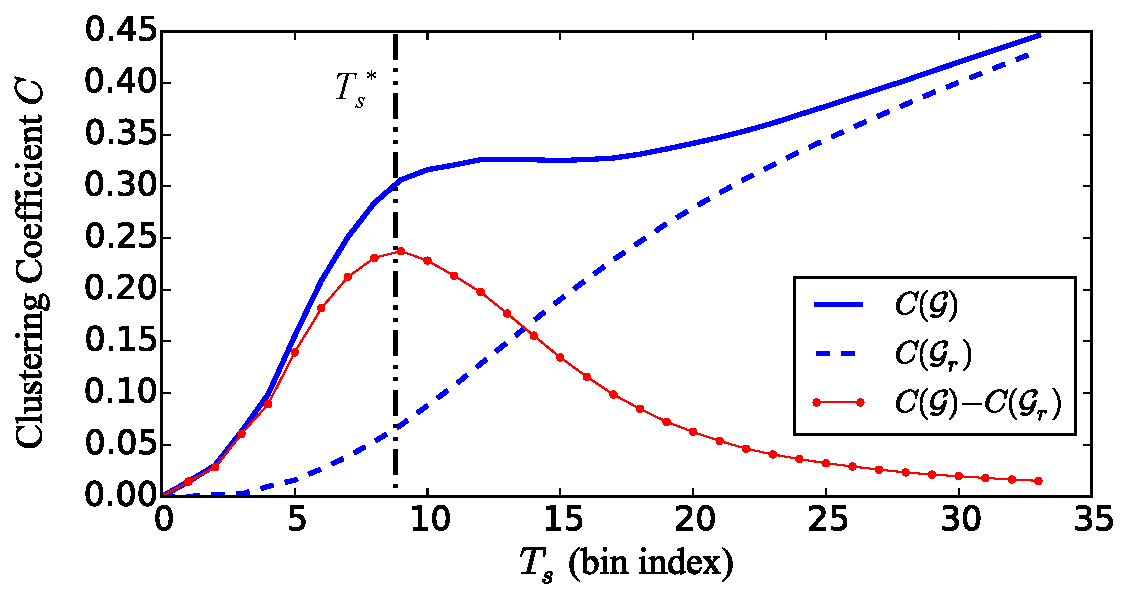
\includegraphics[width=\figSizeEightyFive]{ch07_ragaRecognition/figures/ClusteringCoffs_40raga_2s.pdf}
	\end{center}
	\caption{Evolution of clustering coefficients of $\netUndirWght$ and $\netUndirWght_r$ and their difference for different similarity thresholds~($\simThsld$).}
	\label{fig:raga_rec_clustering_coff_evolution}
\end{figure}

As discussed in~\secref{sec:patterns_characterization_of_melodic_patterns} determining a meaningful similarity threshold in an unsupervised manner is a challenging task. For estimating an optimal value of $\simThsld$ we follow the approach as described in~\secref{sec:network_filtering}. We compare the evolution of the clustering coefficient $\clusCoff$ of the obtained network $\netUndirWght$ with the clustering coefficient of a randomized network $\netUndirWght_r$ over different distance thresholds $\simThsld$. The randomized network $\netUndirWght_r$ is obtained by swapping the edges between randomly selected pairs of nodes such that the degree of each node is preserved~\citep{maslov2002specificity}. The optimal threshold $\simThsld^\star$ is taken as the distance that maximizes the difference between the two clustering coefficients.  In~\figref{fig:raga_rec_clustering_coff_evolution}, we show $\clusCoff(\netUndirWght)$, $\clusCoff(\netUndirWght_r)$ and $\clusCoff(\netUndirWght)-\clusCoff(\netUndirWght_r)$ for different values of $\simThsld$, and mark the optimal threshold $\simThsld^\star$.

The next step of our method we group together similar melodic patterns~(\figref{fig:bd_phasebased_raga_recognition}). To do so, we detect non-overlapping communities in the network of melodic patterns using the method proposed by~\cite{blondel2008fast}. This community detection method is based on optimizing the modularity of the network and is parameter-free from the user's point of view. This method is capable of handling very large networks and has been extensively used in various applications~\citep{fortunato2010community}. We use its implementation available in networkX~\citep{hagberg-2008-exploring}, a Python language package for exploration and analysis of networks and network algorithms. Note that, from now on, the melodic patterns grouped within a community are regarded as the occurrences of a single melodic phrase. Thus, a community essentially represents a melodic phrase or motif.


\subsubsection{TFIDF Feature Extraction}
\label{sec:vsm_feature_extraction_TFID_computation}

As mentioned above, we draw an analogy between \gls{raga} rendition and textual description of a topic. Using this analogy we represent each audio recording using a vector space model, wherein melodic patterns are considered as words (or terms). This process is divided into three blocks (Figure~\ref{fig:bd_phasebased_raga_recognition}).

We start by building our vocabulary $\pattVocab$, which translates to selecting relevant pattern communities for characterizing \glspl{raga}. For this, we include all the detected communities except the ones that comprise patterns extracted from only a single audio recording. Such communities are analogous to the words that only occur within a document and, hence, are irrelevant for modeling a topic.%The size of the obtained vocabulary $\pattVocab$ corresponding to the optimal threshold mentioned above ($\simThsld^\star=9$) is XXX.

We experiment with three different sets of features $\featureVSMOne$, $\featureVSMTwo$ and $\featureVSMThree$, which are similar to the \gls{tfidf} features typically used in text information retrieval. We denote our corpus by $\corpus$  comprising $\nRecCorpus = |\corpus|$ number of recordings. A melodic phrase and a recording is denoted by $\pattern$ and $\recording$ , respectively

\begin{equation}
\featureVSMOne(\pattern,\recording)= 
\begin{cases}
1				,& \text{if}~~\feaqPhRec(\pattern,\recording) > 0\\
0,              & \text{otherwise}
\end{cases}
\end{equation}
where, $\feaqPhRec(\pattern,\recording)$ denotes the raw frequency of occurrence of pattern $\pattern$ in recording $\recording$. $\featureVSMOne$ only considers the presence or absence of a pattern in a recording. In order to investigate if the frequency of occurrence of melodic patterns is relevant for characterizing \glspl{raga}, we take $\featureVSMTwo(\pattern,\recording) = \feaqPhRec(\pattern,\recording)$. As mentioned, the melodic patterns that occur across different \glspl{raga} and in several recordings are futile for \gls{raga} recognition. Therefore, to reduce their effect in the feature vector we employ a weighting scheme, similar to the inverse document frequency ($\mathrm{idf}$) weighting in text retrieval.
\begin{equation}
\featureVSMThree(\pattern,\recording) = \feaqPhRec(\pattern,\recording) \times \irf(\pattern,\corpus)
\end{equation}
\begin{equation}
\irf(\pattern,\corpus) = \log \left( \frac{\nRecCorpus}{ |\lbrace \recording \in \corpus: \pattern \in \recording \rbrace|} \right)
\end{equation}
where, $|\lbrace \recording \in \corpus: \pattern \in \recording \rbrace|$ is the number of recordings where the melodic pattern $\pattern$ is present, that is $\feaqPhRec(\pattern,\recording)\neq 0$ for these recordings. 


\TODO{Only if you are reporting the results from these variants include them here, otherwise comment this para.}
The number of melodic patterns obtained from an audio recording tends to be proportional to the length of the recording. In order to reduce the affect of different recording lengths, we investigate two feature vector normalization techniques frequently used in text classification. In addition to using raw features vectors we experiment with $\mathrm{L}_1$ and $\mathrm{L}_2$ normalization~\cite{leopold2002text}.\TODO{A better reference, also report results corresponding to this?}. 

\COMMENT{is it possible to draw any figure that would make the understanding of this feature very easy? like the one you used in presentations.}


\subsection{Evaluation}
\label{sec:raga_rec_pattern_evaluation}

\subsubsection{Music Collection}
\label{sec:raga_rec_pattern_music_collection}

The music collection used for evaluation in this study is a subset of the CompMusic Carnatic music corpus (\secref{sec:corpus_carnatic_music_corpus}). Due to the differences in the melodic characteristics of Carnatic and Hindustani music, to evaluate our method we compile and curate two datasets, \acrshort{rrds_cmd_big} and \acrshort{rrds_hmd_big}, one for each music tradition. A separate evaluation on both the music traditions allows a better analysis and interpretation of the results.

\acrshort{rrds_cmd_big} and \acrshort{rrds_hmd_big} comprise 124 and 130\,hours of commercially available audio recordings, respectively. All the editorial metadata for each audio recording is publicly available in Musicbrainz\footnote{https://musicbrainz.org/}, an open-source metadata repository. \acrshort{rrds_cmd_big} contains full-length recordings of 480~performances belonging to 40~\glspl{raga} with 12~music pieces per \gls{raga}. \acrshort{rrds_hmd_big} contains full-length recordings of 300~performances belonging to 30~\glspl{raga} with 10~music pieces per \gls{raga}. The selected music material is diverse in terms of the number of artists, the number of forms, and the number of compositions, and thus,  it is representative of these music traditions. The chosen \glspl{raga} contain diverse sets of \glspl{svara}, both in terms of the number of \glspl{svara} and their pitch-classes (\glspl{svarsthana}).

To the best of our knowledge these are the largest and the most comprehensive (in terms of the available metadata) datasets ever used for studying the task of automatic \gls{raga} recognition. To facilitate reproducible research and comparative studies we also make these datasets publicly available online (\appref{app:resources}). A further detailed description of these datasets is provided in~\secref{sec:corpus_raga_recognition_datasets}. 

\subsubsection{Classification and Evaluation Methodology}
\label{sec:raga_rec_pattern_classification_evaluation}

The features obtained above are used to train a classifier. In order to assess the relevance of these features for \gls{raga} recognition, we experiment with different algorithms exploiting diverse classification strategies~\citep{Hastie09BOOK}: \acrfull{nbm}, \acrfull{nbg}, and \acrfull{nbb}, support vector machines with a linear and a radial basis function kernel, and with a stochastic gradient descent learning (\acrshort{svml}, \acrshort{svmr} and \acrshort{sgd}, respectively), \acrfull{lr} and \acrfull{randforest}. We use the implementation of these classifiers available in scikit-learn toolkit~\citep{scikitlearn}, version 0.15.1. Since in this study, our focus is to extract a musically relevant set of features based on melodic patterns, we use the  default parameter settings for the classifiers available in scikit-learn. 

We use leave-one-out cross validation methodology for evaluations~\citep{Mitchell97BOOK}, in which one recording in the evaluation dataset forms the testing set and the remaining ones become the training set. We use the mean classification accuracy across recordings as the evaluation measure. To assess if the difference in the performance between any two methods is statistically significant, we use McNemar's test~\citep{mcnemar1947note} with $p < 0.01$. In addition, to compensate for multiple comparisons, we apply the Holm-Bonferroni method~\citep{holm1979simple}. 

Note that in our published work in~\cite{gulatiphrase_2016} we use a different evaluation strategy (12-fold cross-validation methodology). Therefore the results provided in the article differ slightly form the ones presented in this thesis. In addition, the method for assessing statistical significance is also different (Mann-Whitney U test), which is due to the difference in the evaluation strategy. The evaluation strategy used here (eave-one-out cross validation) does not involve any random sampling (or split) of the evaluation set, which makes our experimental setup more definite.

\subsubsection{Comparison with the State-of-the-art}
\label{sec:raga_rec_pattern_comparison_sota}

We compare our results with two state-of-the-art methods proposed in~\citep{chordia2013joint} and \citep{koduri2014intonation}. As an input to these methods, we use the same features, predominant pitch and tonic, as used in our method. The only difference is that the pitch contours fed to these methods are not post-processed (\secref{sec:data_preprocessing_pitch_postprocessing}). This is because these methods primarily exploit the intonation aspect of the \glspl{svara}, and therefore, performing a smoothening operation on pitch contours might degrade their performance. The method in~\cite{chordia2013joint} uses smoothened \acrfull{pcd} as the tonal feature and employs \acrfull{1nn} using Bhattacharyya distance for predicting \gls{raga} labels. We denote this method by \acrshort{sotaChordia}. The authors in~\cite{chordia2013joint} report a window size of 120\,s as an optimal duration for computing \glspl{pcd} (denoted here by $\mathrm{PCD}_{120}$). However, in our experiments we find that \glspl{pcd} computed over the entire audio recording (denoted here by~$\mathrm{PCD}_\mathrm{full}$) result in a significant improvement~\citep{gulatiphrase_2016}. We therefore use $\mathrm{PCD}_\mathrm{full}$ for comparison. Note that in~\cite{chordia2013joint} the authors do not experiment with a window size larger than 120\,s. 

The method in~\cite{koduri2014intonation} is proposed primarily for Carnatic music. This method also uses features based on pitch distribution. However, unlike in \acrshort{sotaChordia}, the authors use parameterized pitch distribution of individual \glspl{svara} as features (denoted here by $\mathrm{PD}_\mathrm{param}$). We denote this method by \acrshort{sotaKoduri}. Note that \acrshort{sotaKoduri} utilizes specific intonation aspects of \glspl{svara} in Carnatic music, and is not devised to work with Hindustani music recordings. We therefore do not consider this method for comparing results on Hindustani music. The authors of both these papers courteously ran the experiments on our dataset using the original implementations of the methods. 


\subsection{Results and Discussion[SIGNIFICANT WORK TBD]}
\label{sec:vsm_eval_results}

\TODO{1) Table with latest results, 2) CC curve against performance accuracy, 3) Confusion matrices of our approach and sota approaches, 4) Statistical sig 5) analysis of results and writing them.}

\begin{table}
	\tabcolsep=.18cm
	\centering
	\begin{tabular}{c|c|c|c c c c c}
		\hline
		db & Mtd & Ftr & \acrshort{nbm} & \acrshort{nbb} & \acrshort{lr} & \acrshort{svml} & \acrshort{1nn}\tabularnewline
		\hline \hline 
		\multirow{5}{*}{\begin{turn}{90}DB10r\={a}ga\end{turn}} & \multirow{3}{*}{\acrshort{ragarecVSM}} & $\featureVSMOne$ & 90.6 & 74 & 84.1 & 81.2 & -\tabularnewline
		
		&  & $\featureVSMTwo$ & {\bf 91.7} & 73.8 & 84.8 & 81.2 & -\tabularnewline
		
		&  & $\featureVSMThree$ & 90.5 & 74.5 & 84.3 & 80.7 & -\tabularnewline
		\cline{2-8} 
		& \multirow{2}{*}{\acrshort{sotaChordia}} & $\mathrm{PCD}_{120}$ & - & - & - & - & 82.2\tabularnewline
		& & $\mathrm{PCD}_\mathrm{full}$ & - & - & - & - & {\bf 89.5}\tabularnewline
		\cline{2-8} 
		& \acrshort{sotaKoduri} & $\mathrm{PD}_\mathrm{param}$ & 37.9 & 11.2 & {\bf 70.1} & 65.7 & -\tabularnewline
		\hline \hline
		\multirow{5}{*}{\begin{turn}{90}DB40r\={a}ga\end{turn}} & \multirow{3}{*}{\acrshort{ragarecVSM}} & $\featureVSMOne$ & 69.6 & 61.3 & 55.9 & 54.6 & -\tabularnewline
		
		&  & $\featureVSMTwo$ & {\bf 69.6} & 61.7 & 55.7 & 54.3 & -\tabularnewline
		
		&  & $\featureVSMThree$ & 69.5 & 61.5 & 55.9 & 54.5 & -\tabularnewline
		\cline{2-8} 
		& \multirow{2}{*}{\acrshort{sotaChordia}} & $\mathrm{PCD}_{120}$ & - & - & - & - & 66.4\tabularnewline
		
		& & $\mathrm{PCD}_\mathrm{full}$ & - & - & - & - & {\bf 74.1}\tabularnewline
		\cline{2-8} 
		& \acrshort{sotaKoduri} & $\mathrm{PD}_\mathrm{param}$ & 20.8 & 2.6 & {\bf 51.4} & 44.2 & -\tabularnewline
		\hline \hline
	\end{tabular}
	
	\caption{Accuracy (in percentage) of different methods (Mtd) for two datasets (db) using different classifiers and features (Ftr).} 
	\label{tab:accuracies_for_variants}
\end{table}



In Table~\ref{tab:accuracies_for_variants}, we present the results of our proposed method \acrshort{ragarecVSM} and the two state of the art methods \acrshort{sotaChordia} and \acrshort{sotaKoduri} for the two datasets DB10r\={a}ga and DB40r\={a}ga. The highest accuracy for every method is highlighted in bold for both the datasets. Due to lack of space we present results only for the best performing classifiers. 

We start by analyzing the results of the variants of \acrshort{ragarecVSM}. From Table~\ref{tab:accuracies_for_variants}, we see that the highest accuracy obtained by \acrshort{ragarecVSM} for DB10r\={a}ga is 91.7\%. Compared to DB10r\={a}ga, there is a significant drop in the performance of every variant of \acrshort{ragarecVSM} for DB40r\={a}ga. The best performing variant in the latter achieves 69.6\% accuracy. We also see that for both the datasets, the accuracy obtained by \acrshort{ragarecVSM} across the feature sets is nearly the same for each classifier, with no statistically significant difference. This suggests that, considering just the presence or the absence of a melodic pattern, irrespective of its frequency of occurrence, is sufficient for \gls{raga} recognition. Interestingly, this finding is consistent with the fact that characteristic melodic patterns are unique to a \gls{raga} and a single occurrence of such patterns is sufficient to identify the \gls{raga}~\cite{krishna2012carnatic}. As seen in Table~\ref{tab:accuracies_for_variants}, the performance of the proposed method is very sensitive to the choice of the classifier. We notice that for both the datasets, the best accuracy is obtained using the NBM classifier, and the difference in its performance compared to any other classifier is statistically significant. Note that, the NBM classifier outperforming other classifiers is also well recognized in the text classification community~\cite{mccallum1998comparison}. We, therefore, only consider the NBM classifier for comparing \acrshort{ragarecVSM} with the other methods. It is worth noting that the feature weights assigned by a classifier can be used to identify the relevant melodic patterns for \gls{raga} recognition. These patterns can serve as a dictionary of semantically-meaningful melodic units for many computational tasks in IAM.

In order to validate that the estimated similarity threshold $\simThsld^\star$ (Section~\ref{pattern_clustering}) produces the optimal results, we perform \gls{raga} recognition using different similarity thresholds $\simThsld$. 

\begin{figure}
	\begin{center}
		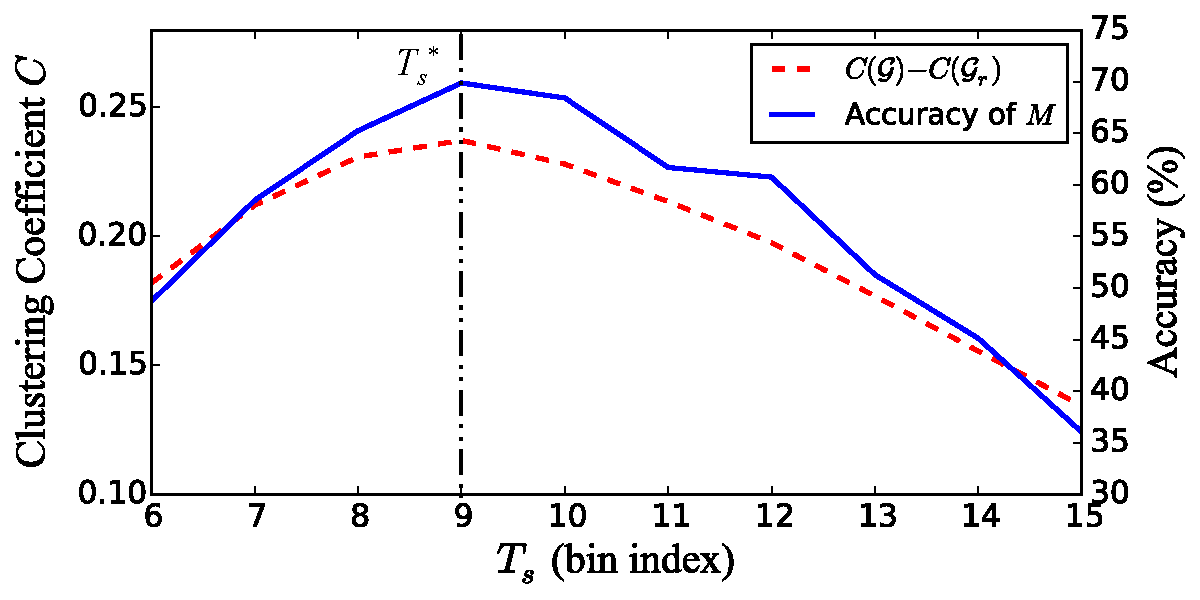
\includegraphics[width=\figSizeEighty]{ch07_ragaRecognition/figures/accuracy_Vs_thresold.pdf}
	\end{center}
	\caption{Accuracy of \acrshort{ragarecVSM} and $\clusCoff(\netUndirWght)-\clusCoff(\netUndirWght_r)$ for different similarity thresholds.}
	\label{fig:performance_across_thresholds}
\end{figure}

\begin{figure}
	\begin{center}
		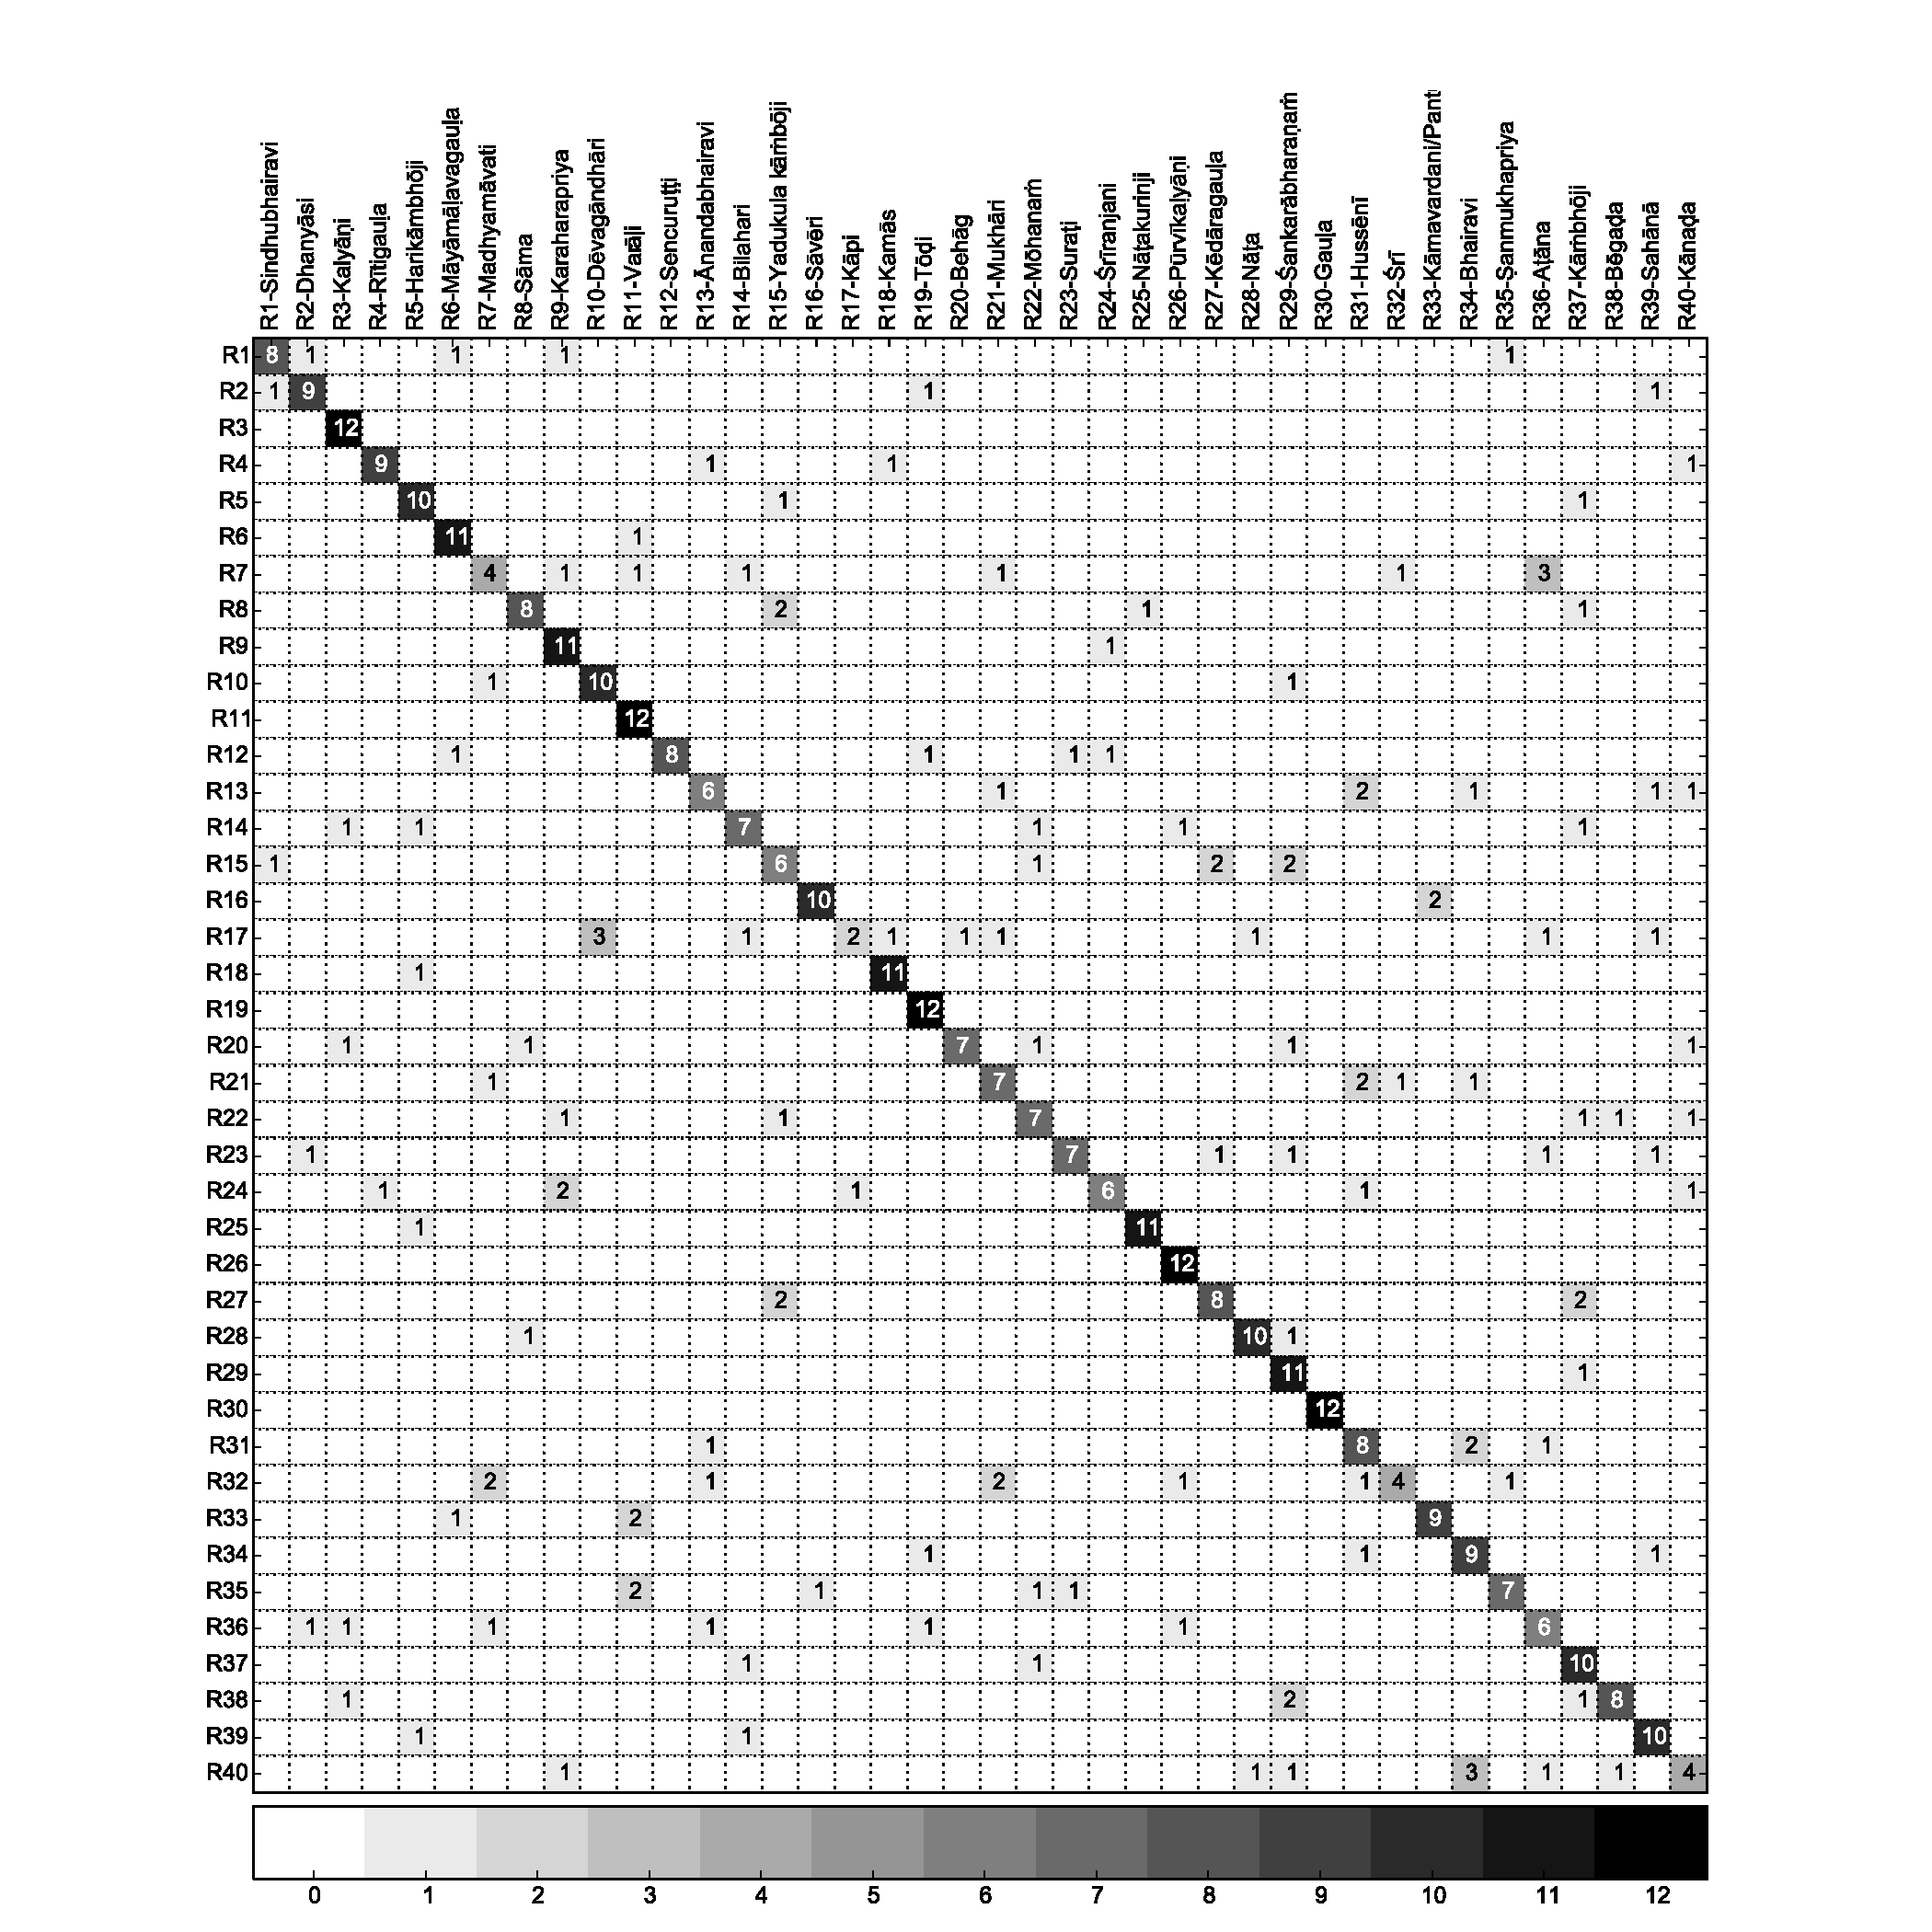
\includegraphics[width=\figSizeHundred]{ch07_ragaRecognition/figures/cnf_mtx_40raga_with_annotation.pdf}
	\end{center}
	\caption{Confusion matrix for the proposed method. The different shades of grey are mapped to different number of audio recordings.}
	\label{fig:confusion_matrix}
\end{figure}

Before further analyses of our results, we verify here our approach to obtain the optimal similarity threshold $\simThsld^\star$ (Section~\ref{pattern_clustering}). In Figure~\ref{fig:performance_across_thresholds}, we show the accuracy obtained by \acrshort{ragarecVSM}, and  $C(\netUndirWght)-C(\netUndirWght_r)$ as a function of similarity threshold $\simThsld$. We see that these curves are highly correlated. Thus, the optimal threshold $\simThsld^\star$, which we defined in Section~\ref{pattern_clustering} as the distance that maximizes the difference $C(\netUndirWght)-C(\netUndirWght_r)$, also results in the best accuracy for \gls{raga} recognition.

We now analyze the confusion matrix, and understand the type of classification errors made by \acrshort{ragarecVSM}, (Figure~\ref{fig:confusion_matrix}). We observe that our method achieves near-perfect accuracy for several \glspl{raga} including Kaly\={a}\d{n}i, P\={u}rvikaly\={a}\d{n}i, T\={o}\d{d}i and Var\={a}\d{l}i. This is consistent with the fact that these are considered to be phrase-based \glspl{raga}, that is, their identity is predominantly derived from melodic phraseology~\cite{krishna2012carnatic}. At the same time, we observe low accuracy for some other phrase-based \glspl{raga} such as Madhyam\={a}vati, K\={a}na\d{d}a and \'{S}r\={i}. On investigating further we find that such \glspl{raga} are confused often with their allied \glspl{raga}\footnote{Allied \glspl{raga} have a common set of svaras and similar melodic movement}~\cite{krishna2012carnatic}. Distinguishing between allied \glspl{raga} is a challenging task, since it is based on subtle melodic nuances. We also note that, among the other \glspl{raga} for which the obtained accuracy is low, several are considered as scale-based \glspl{raga}. This is in line with~\cite{krishna2012carnatic}, where the authors remark that the identification of such \glspl{raga} is not based on melodic phraseology. Overall, this analysis of the classification errors indicates that our proposed method is more suitable for recognizing phrase-based \glspl{raga} compared to scale-based \glspl{raga}. 


Finally, we compare \acrshort{ragarecVSM} with the state of the art methods \acrshort{sotaChordia} and \acrshort{sotaKoduri}. From Table~\ref{tab:accuracies_for_variants}, we see that \acrshort{ragarecVSM} outperforms \acrshort{sotaKoduri} for both the datasets, and the difference is found to be statistically significant. When compared with \acrshort{sotaChordia}, we see that \acrshort{ragarecVSM} performs significantly better than the $\mathrm{PCD}_{120}$ variant of \acrshort{sotaChordia} for both the datasets. However, the performance of the $\mathrm{PCD}_\mathrm{full}$ variant of \acrshort{sotaChordia} is comparable to \acrshort{ragarecVSM} for DB10r\={a}ga, and, significantly better for DB40r\={a}ga. A comparison of the results of \acrshort{ragarecVSM} and \acrshort{sotaChordia} for each \gls{raga} reveals that their performance is complementary. \acrshort{ragarecVSM} successfully recognizes several \glspl{raga} with high accuracy for which \acrshort{sotaChordia} performs poorly, and vice-versa. This suggests that the proposed pattern-based method can be combined with the pitch distribution-based methods to achieve a higher \gls{raga} recognition accuracy.



\section{\titlecap{\glsentrylong{tdms} for \glsentrytext{raga} recognition}}
\label{sec:tdms_raga_recognition}

The method described in the previous section (\acrshort{ragarecVSM}) uses melodic patterns to perform \gls{raga} recognition (\secref{sec:phrase_based_feature_extraction}). Using automatically discovered short-duration melodic patterns that constitute only a fraction of the total duration of the audio recordings, \acrshort{ragarecVSM} shows promising results by achieving an accuracy comparable to the state-of-the-art method. While we further refine our methodology for discovering melodic patterns and in turn improve \gls{raga} recognition, we also propose another method, \acrshort{ragarecTDMS}, for this task. 

Similar to \acrshort{ragarecVSM}, \acrshort{ragarecTDMS} aims to capture the tonal and the temporal characteristics of melody by using its continuous representation. However, instead of using short-duration patterns extracted directly from the surface representation of melody as done in \acrshort{ragarecVSM}, in \acrshort{ragarecTDMS} we seek to abstract the melody representation. An abstraction of melody that imbibes both the tonal and the temporal aspects relates to the concept of \gls{chalan} in \gls{iam} (\secref{sec:melody_in_iam}). \Gls{chalan} (literally meaning gait or movement) of a \gls{raga} defines its melodic outline in terms of how a melodic transition is to be made from one \gls{svara} to another, the precise intonation to be followed, and the proportion of time spent on each \gls{svara}. \Gls{chalan} can be considered as an abstraction of \gls{raga} motifs, and is a characterizing feature of \glspl{raga}. \acrshort{ragarecTDMS} utilizes \gls{chalan} aspect of melodies in \gls{iam} to perform \gls{raga} recognition.

In order to abstract the continuous melody representation and incorporate \gls{chalan} aspects, \acrshort{ragarecTDMS} uses a novel feature,  the \acrfull{tdms}. \gls{tdms} captures tonal and temporal melodic aspects that are useful in characterizing and distinguishing \glspl{raga}. \Glspl{tdms} alleviate several of the shortcomings in the existing approaches (\secref{sec:sota_raga_recognition}) and improves the accuracy of \gls{raga} recognition by large margins. \Gls{tdms} is inspired by the concept of delay coordinates~\citep{takens1981detecting}. The main strengths of \gls{tdms} are:

\begin{itemize}
	\item It is a compact representation that describes both the tonal and the temporal characteristics of a melody
	\item It simultaneously captures the melodic characteristics at different time-scales, the overall usage of the pitch-classes in the entire recording, and the short-time temporal relation between individual pitches.
	\item It is robust to pitch octave errors.
	\item It does not require the transcription of the melody nor a discrete representation of it.
	\item It is easy to implement, fast to compute, and has a musically-meaningful interpretation.
	\item As it will be shown, it obtains unprecedented accuracies in the raga recognition task, outperforming the state-of-the-art by a large margin, without the use of any elaborated classification schema.
\end{itemize}

We now proceed to describe \acrshort{ragarecTDMS},.which is largely based on the \gls{tdms} features. The computation of \gls{tdms} is described in the subsequent section (\secref{sec:tdms_feature_extraction}). The classification strategy and the distance measure used on top of the \gls{tdms} features for recognizing \glspl{raga} are described in~\secref{sec:tdms_classification_evaluation}. In~\secref{sec:tdms_eval_results}, we present the experimental setup used to evaluate this method, and finally, discuss the obtained results. 

\subsection{\titlecap{\glsentrylong{tdms}}}
\label{sec:tdms_feature_extraction}

\begin{figure}
	\begin{center}
		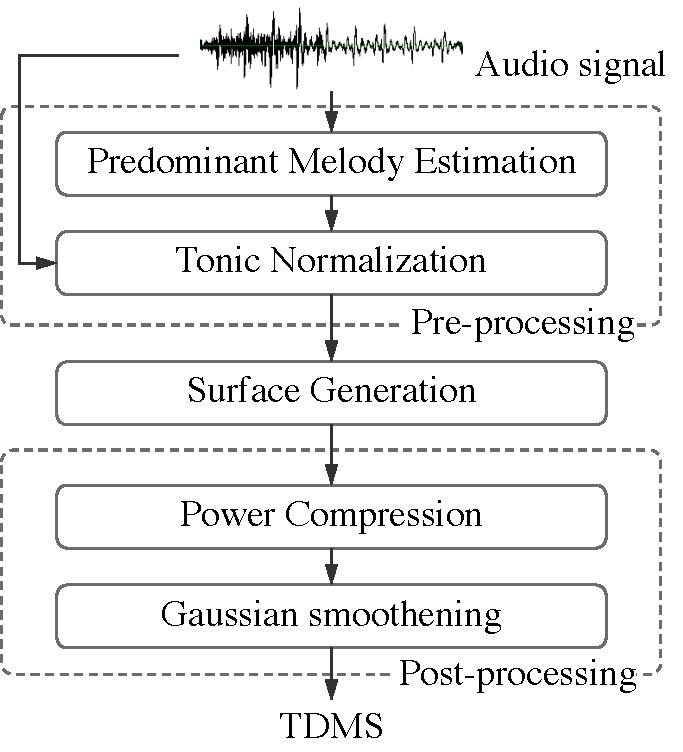
\includegraphics[width=\figSizeFifty]{ch07_ragaRecognition/figures/tdms_computation.pdf}
	\end{center}
	\caption{Block diagram for \gls{tdms} computation.\TODO{replace melody by pitch}}
	\label{fig:bd_tdms_computation}
\end{figure}

The computation of a \gls{tdms} involves three steps as shown in~\figref{fig:bd_tdms_computation}: pre-processing, surface generation, and post-processing. In the pre-processing step, we obtain a low-level representation of the melody from an audio recording, which is then put to a meaningful tonal context by normalizing it with respect to the tonic pitch of the recording. In the surface generation step, we compute a two dimensional surface based on the concept of delay coordinates. Finally, in the post-processing step, we apply power compression and Gaussian smoothing to the computed surface. All these processing steps are described in the subsequent sections.

\subsubsection{Pre-processing} 
\label{sec:tdms_preprocessing}

\paragraph{Predominant Pitch Estimation}

In this step we process an audio recording to obtain a low-level representation of the melody, which is subsequently used in the computation of the \gls{tdms}. For this, we consider predominant pitch in the audio signal as the low-level melody representation. For predominant pitch estimation we follow the method described in~\secref{sec:data_preprocessing_predominant_melody_estimation}. In addition, we also post-process the estimated pitch to smoothen it and remove spurious pitch jumps (\secref{sec:data_preprocessing_pitch_postprocessing}). \TODO{params for both pitch and post processing.}

\paragraph{Tonic Normalization}

The base frequency chosen in a performance of \gls{iam} is the tonic pitch of the lead artist, to which all other accompanying instruments are tuned~(\secref{sec:melody_in_iam}). 
Tonic pitch varies across artists and their recordings, and therefore, a meaningful feature for \gls{raga} recognition should be normalized with respect to the tonic pitch. To achieve this, we normalize the predominant pitch of every recording by considering its tonic pitch as the reference frequency during the Hertz-to-Cent-scale conversion~(\secref{sec:pre_processing_melody_representation}). The tonic pitch of the lead artist for every recording is automatically identified using \acrshort{tonicid_justin}, the method that outperformed all other existing methods for this task as shown in our comparative evaluation~(\secref{sec:pre_processing_tonic_identification_summary}). 

\subsubsection{Surface Generation}
\label{sec:tdms_surface_generation}

The next step is to construct a two-dimensional surface based on the concept of delay coordinates (also termed phase space embedding)~\citep{takens1981detecting, Kantz04BOOK}. In fact, such two-dimensional surface can be seen as a discretized histogram of the elements in a two-dimensional Poicar\'e map~\citep{Kantz04BOOK}. For a given recording, we generate a surface $\tdmsBase$ of size $\sizeTDMS\times\sizeTDMS$ recursively, by computing

\begin{equation}
\label{eq:surface_computation1}	
\tdmsElem_{ij} = \sum_{t=\timeDelay}^{N-1} \indFnc\left(\binOp\left(\pitchCents_t\right),i\right)~ \indFnc\left(\binOp\left(\pitchCents_{t-\timeDelay}\right),j\right) 
\end{equation}

for $0 \leq i,j < \sizeTDMS$, where $\tdmsElem_{ij}$ is the $(i,j)^\mathrm{th}$ element of the two-dimensional matrix $\tdmsBase$, $\pitchCents_t$ is the $t^\mathrm{th}$ sample (in Cent-scale) of the pitch sequence of length $N$, $\indFnc$ is an indicator function such that

\begin{equation}
\begin{aligned}
\indFnc(x,y)=
\begin{cases}
1, & \text{iff } x=y\\
0, & \text{otherwise}
\end{cases}
\end{aligned}
\end{equation}
 
$\binOp$ is an octave-wrapping integer binning operator defined by
 
\begin{equation}	
\label{eq:binning_function}	
\binOp(x) = \left\lfloor ~\left(\frac{\sizeTDMS x}{1200}\right) \bmod \sizeTDMS ~\right\rfloor,
\end{equation}

and $\timeDelay$ is a time delay index (in frames) that is left as a parameter. Note that, the frames where a predominant pitch could not be obtained (unvoiced segments) are excluded from any calculation. For the size of $\tdmsBase$ we use $\sizeTDMS = 120$. This value  corresponds to 10 cents per bin, an optimal pitch resolution reported in~\citep{chordia2013joint}. The study shows that \gls{raga} recognition using \glspl{pcd} with a bin width of 10\,Cents outperforms the \glspl{pcd} with a bin width of 100\,Cents, and obtains a comparable results to \glspl{pcd} with a bin width of 5\,Cents.

An example of the generated surface $\tdmsBase$ for a music piece\footnote{\url{http://musicbrainz.org/recording/e59642ca-72bc-466b-bf4b-d82bfbc7b4af}} in \gls{raga} Yaman is shown in~\figref{fig:phase_space_surface}\,(a). We see that the prominent peaks in the surface correspond to the \glspl{svara} of \gls{raga} Yaman. We notice that these peaks are steep and the dynamic range of the surface is high. This can be attributed to the nature of the melodies in these music traditions, particularly in Hindustani music, where the melodies often contain long held \glspl{svara}. In addition, the dynamic range is high also because the pitches in the stable \gls{svara} regions lie within a small frequency range around the mean \gls{svara} frequency compared to the pitches in the transitory melodic regions. Because of this, most of the pitch values are mapped to a small number of bins, making the prominent peaks more steep.

\begin{figure}[t]
	\begin{center}
		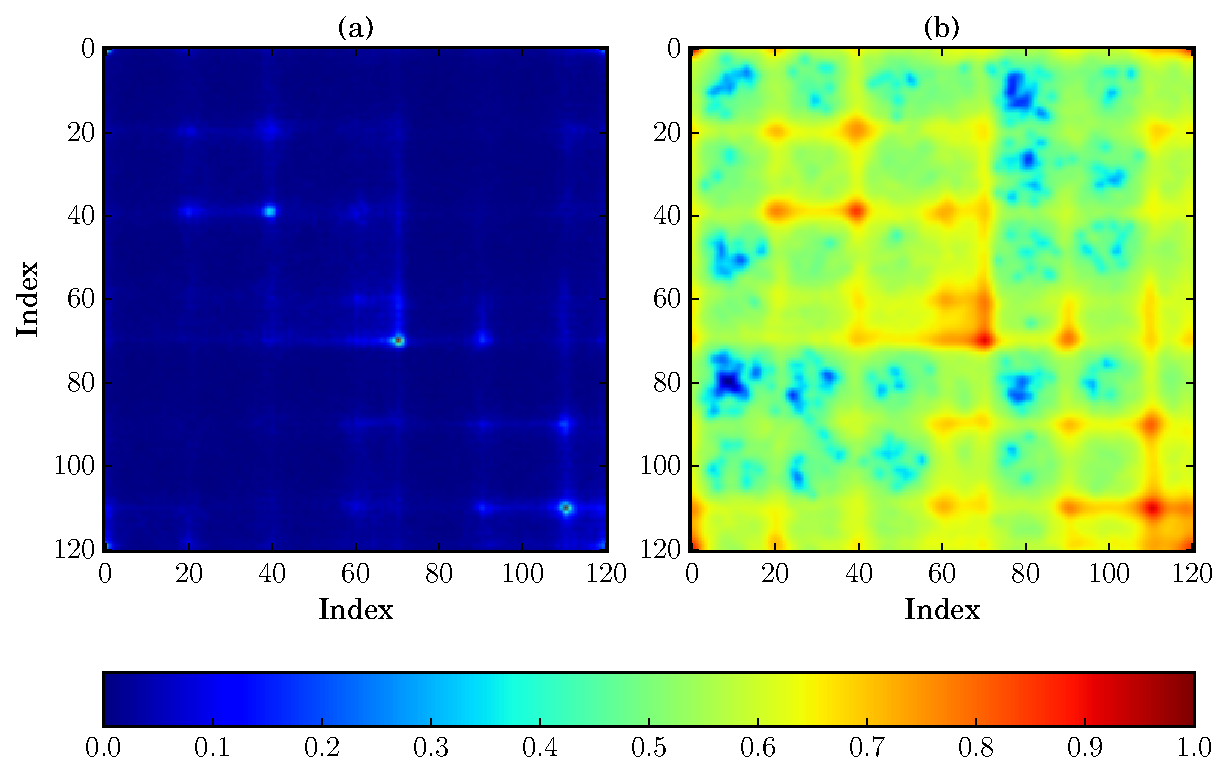
\includegraphics[width=\figSizeEighty]{ch07_ragaRecognition/figures/PSfeature_e59642ca-72bc-466b-bf4b-d82bfbc7b4af.pdf}
	\end{center}\vspace{-1.5em}
	\caption{Generated surface for a music piece before (a) and after (b) applying post-processing ($\tdmsBase$ and $\tdmsSmooth$, respectively). For ease of visualization, both matrices are normalized here between 0 and 1.}
	\label{fig:phase_space_surface}
	\vspace{-0.5em}
\end{figure}

\subsubsection{Post-processing}
\label{sec:tdms_post_processing}

In order to accentuate the values corresponding to the transitory regions in the melody and reduce the dynamic range of the surface, we apply an element-wise power compression
\begin{equation*}
%\label{eq:power_compression}	
\tdmsPower= \tdmsBase^\tdmsPowFac ,
\end{equation*}
where $\tdmsPowFac$ is an exponent that is left as a parameter. Once a more compact (in terms of the dynamic range) surface is obtained, we apply Gaussian smoothing. With that, we attempt to attenuate the subtle differences in $\tdmsPower$ corresponding to the different melodies within the same \gls{raga}, while retaining the attributes that characterize that \gls{raga}. 

We perform Gaussian smoothing by circularly convolving $\tdmsPower$ with a two-dimensional Gaussian kernel. We choose a circular convolution because of the cyclic (or octave-folded) nature of the \gls{tdms} (Equation~\ref{eq:binning_function}), which mimics the cyclic nature of pitch classes. The standard deviation of this kernel is $\sigma$ bins (samples). The length of the kernel is truncated to $8\sigma + 1$ bins in each dimension, after which the values are negligible (below $0.01\%$ of the kernel's maximum amplitude). We experiment with different values of $\sigma$, and also with a method variant excluding the Gaussian smoothing (loosely denoted by $\sigma = -1$), so that we can quantify its influence on the accuracy of the system. 
%
%After convolution we retain the same dimensionality of the surface as before by discarding $4\sigma$ number of samples from the start and the end of each dimension (i.e.~the border). 

Once we have the smoothed surface $\tdmsSmooth$, there is only one step remaining to obtain the final \gls{tdms}. Since the overall duration of the recordings and of the voiced regions within them is different, the computed surface $\tdmsSmooth$ needs to be normalized. To do so, we divide $\tdmsSmooth$ by its $L_1$ matrix norm:
\begin{equation*}
\tdmsNorm = \tdmsSmooth/\norm{\tdmsSmooth}_{1} .
\end{equation*}
This also yields values of $\tdmsNorm$, the final TDMS, that are interpretable in terms of discrete probabilities.

The result after post-processing the surface of Figure~\ref{fig:phase_space_surface}\,(a) with power compression and Gaussian smoothing is shown in Figure~\ref{fig:phase_space_surface}\,(b). We see that the values corresponding to the non-diagonal elements are accentuated. A visual inspection of Figure~\ref{fig:phase_space_surface}\,(b) provides several musical insights to the melodic aspects of the recording. For instance, the high salience indices along the diagonal, $(0,0)$, $(20,20)$, $(40,40)$, $(60,60)$, $(70,70)$, $(90,90)$, and $(110,110)$, correspond to the 7~svaras used in \gls{raga} Yaman. Within which, the highest salience at indices (110,110) correspond to the Ni svara, which is the {\it Vadi} svara, i.e., musically the most salient svara of the \gls{raga}, in this case \gls{raga} Yaman~\cite{rao1999raga}. The asymmetry in the matrix with respect to the diagonal indicates the asymmetric nature of the ascending and descending svara pattern of the \gls{raga} (compare, for example, the salience at indices $(70, 90)$ to indices $(90, 70)$, with the former being more salient than the latter). The similarity of the matrix between indices $(20,20)$ and $(70,70)$ with respect to the matrix between indices $(70,70)$ and $(120,120)$ delineates the tetra-chord structure of the \gls{raga}. Finally, it should be noted that an interesting property of TDMSs is that the mean of the sum across its row and columns yields a PCD representation (see Section \TODO{XXX}).

\subsection{Classification and Distance Measures}
\label{sec:tdms_classification_evaluation}

In order to demonstrate the ability of the \gls{tdms} s in capturing \gls{raga} characteristics, we consider the task of classifying audio recordings according to their \gls{raga} label. To perform classification, we choose a $k$-nearest neighbor (kNN) classifier~\cite{Mitchell97BOOK}. The reasons for our choice are manifold. Firstly, the kNN classifier is well understood, with well studied relations to other classifiers in terms of both performance and architecture. Secondly, it is fast, with practically no training and with known techniques to speed up testing or retrieval. Thirdly, it has only one parameter, $k$, which we can just blindly set to a relatively small value or can easily optimize in the training phase. Finally, it is a classifier that is simple to implement and whose results are both interpretable and easily reproducible. 

The performance of a kNN classifier highly depends on the distance measure used to retrieve the $k$ neighbors. We consider three different measures to compute the distance between two recordings $n$ and $m$ with \gls{tdms}\ features $\tdmsNorm^{(n)}$ and $\tdmsNorm^{(m)}$, respectively. We first consider the Frobenius norm of the difference between $\tdmsNorm^{(n)}$ and $\tdmsNorm^{(m)}$,
\begin{equation*}
\distTDMS_{\mathrm{F}}^{(n,m)} = \norm{\tdmsNorm_{n} - \tdmsNorm_{m}}_2 .
\end{equation*}
Next, we consider the symmetric Kullback-Leibler divergence
\begin{equation*}
\distTDMS_{\mathrm{KL}}^{(n,m)} = \distTDMS_{\mathrm{KL}}\left(\tdmsNorm^{(n)},\tdmsNorm^{(m)}\right) + \distTDMS_{\mathrm{KL}}\left(\tdmsNorm^{(m)},\tdmsNorm^{(n)}\right) ,
\end{equation*}
with
\begin{equation*}
\distTDMS_{\mathrm{KL}}\left(\mathbf{X},\mathbf{Y}\right) = \sum{\mathbf{X} \log\left(\frac{\mathbf{X}}{\mathbf{Y}} \right)} ,
\end{equation*}
where we perform element-wise operations and sum over all the elements of the resultant matrix. Finally, we consider the Bhattacharyya distance, which is reported to outperform other distance measures with a PCD-based feature for the same task in~\cite{chordia2013joint},
\begin{equation*}
\distTDMS_{\mathrm{B}}^{(n,m)} = -\log\left( \sum{ \sqrt{ \tdmsNorm^{(n)} \cdot \tdmsNorm^{(m)} } } \right) .
\end{equation*}
We again perform element-wise operations and sum over all the elements of the resultant matrix. Variants of our proposed method that use $\distTDMS_{\mathrm{F}}$, $\distTDMS_{\mathrm{KL}}$ and $\distTDMS_{\mathrm{B}}$ are denoted by \acrshort{ragarecTDMS_F}, \acrshort{ragarecTDMS_KL}, and \acrshort{ragarecTDMS_B}, respectively.



\subsection{Evaluation, Results and Discussion}
\label{sec:tdms_eval_results}

To evaluate the performance of the considered methods we use the raw overall accuracy~\cite{Mitchell97BOOK}. Since both CMD and HMD are balanced in the number of instances per class, we do not need to correct such raw accuracies to counteract for possible biases towards the majority class. We perform a leave-one-out cross validation~\cite{Mitchell97BOOK}, in which one recording from the evaluation data set forms the testing set and the remaining ones become the training set. To assess if the difference in the performance between any two methods is statistically significant, we use McNemar's test~\cite{mcnemar1947note} with $\pVal < 0.01$. To compensate for multiple comparisons, we apply the Holm-Bonferroni method~\cite{holm1979simple}. Besides accuracy, and for a more detailed error analysis, we also compute the confusion matrix over the predicted classes.

In the case of \acrshort{ragarecTDMS}, a test recording is assigned the majority class of its $k$-nearest neighbors obtained from the training set and, in case of a tie, one of the majority classes is selected randomly. Because we conjecture that none of the parameters we consider is critical to obtain a good performance, we initially make an educated guess and intuitively set our parameters to a specific combination. We later study the influence of every parameter starting from that combination. We initially use $\timeDelay=0.3$\,s, $\tdmsPowFac=0.75$, $\sigma=2$, and $k=1$, and later consider $\timeDelay\in\lbrace 0.2, 0.3, 0.5, 1, 1.5\rbrace$\,s, $\tdmsPowFac\in\lbrace 0.1, 0.25, 0.5, 0.75, 1 \rbrace$, $\sigma\in\lbrace -1, 1, 2, 3\rbrace$, and $k\in\lbrace 1,3,5\rbrace$ (recall that $\sigma=-1$ corresponds to no smoothing; Section~\TODO{XXX}.


In Table~\ref{tab:main_results}, we show the results for all the variants of the proposed method \acrshort{ragarecTDMS_F}, \acrshort{ragarecTDMS_KL} and \acrshort{ragarecTDMS_B}, and the two state-of-the-art methods \acrshort{sotaChordia} and \acrshort{ragarecVSM}, using HMD and CMD data sets. We see that the highest accuracy obtained on HMD is 97.7\% by \acrshort{ragarecTDMS_KL} and \acrshort{ragarecTDMS_B}. This accuracy is considerably higher than the 91.7\% obtained by \acrshort{sotaChordia}, and the difference is found to be statistically significant. We also see that \acrshort{sotaChordia} performs significantly better than \acrshort{ragarecVSM}. Regarding the proposed variants, we see that, in HMD, \acrshort{ragarecTDMS_KL} and \acrshort{ragarecTDMS_B} perform better than \acrshort{ragarecTDMS_F}, with a statistically significant difference. 

\begin{table}[t] 
	\centering
	{
		\begin{tabular}{ c | c c c | c c}
			\hline\hline
			Dataset   	& 	\acrshort{ragarecTDMS_F} 	&	\acrshort{ragarecTDMS_KL}		&	\acrshort{ragarecTDMS_B}	&	\acrshort{sotaChordia}		&	\acrshort{ragarecVSM}\\	
			\hline
			HMD   	& 	91.3 	&	{\bf 97.7}		&	{\bf 97.7} 	&	91.7		&	83.0\\	
			
			CMD   	& 	81.5	&	{\bf 86.7}		&	{\bf 86.7}	&	73.1		&	68.1\\	
			\hline\hline
		\end{tabular}
	}
	\caption{Accuracy (\%) of the three proposed variants, \acrshort{ragarecTDMS_F}, \acrshort{ragarecTDMS_KL} and $\mathcal{M}_{\mathrm{BC}}$, and the two existing state-of-the-art methods \acrshort{sotaChordia} and \acrshort{ragarecVSM} (see text). The random baseline for this task is 3.3\% for HMD and 2.5\% for CMD. }
	\label{tab:main_results}
\end{table}

In Table~\ref{tab:main_results}, we see that the trend in the performance for  CMD across different methods is similar to that for  HMD. The variants \acrshort{ragarecTDMS_KL} and \acrshort{ragarecTDMS_B} achieve the highest accuracy of 86.7\%, followed by \acrshort{sotaChordia} with 73.1\%. The difference between \acrshort{ragarecTDMS_KL} (\acrshort{ragarecTDMS_B}) and \acrshort{sotaChordia} is found to be statistically significant.  For CMD, also  \acrshort{ragarecTDMS_KL} and \acrshort{ragarecTDMS_B} perform better than \acrshort{ragarecTDMS_F}, with a statistically significant difference. 

In general, we notice that, for every method, the accuracy is higher on HMD compared to CMD. This, as expected, can be largely attributed to the difference in the number of classes in  HMD (30 \glspl{raga}) and  CMD (40 \glspl{raga}). A higher number of classes makes the task of \gls{raga} recognition more challenging for  CMD, compared to  HMD. In addition to that, another factor that can cause this difference could be the length of the audio recordings, which for  HMD are significantly longer than the ones in CMD.

As mentioned earlier, the system parameters corresponding to the results in Table~\ref{tab:main_results} were set intuitively, without any parameter tuning. Since \gls{tdms} s are used here for the first time, we want to carefully analyze the influence that each of the parameters has on the final \gls{raga} recognition accuracy, and ultimately perform a quantitative assessment of their importance. In Figure~\ref{fig:accuracy_vs_parameter_values}, we show the accuracy of \acrshort{ragarecTDMS_KL} for different values of these parameters. In each case, only one parameter is varied and the rest are set to the initial values mentioned above. 

\begin{figure}[t]
	\begin{center}
		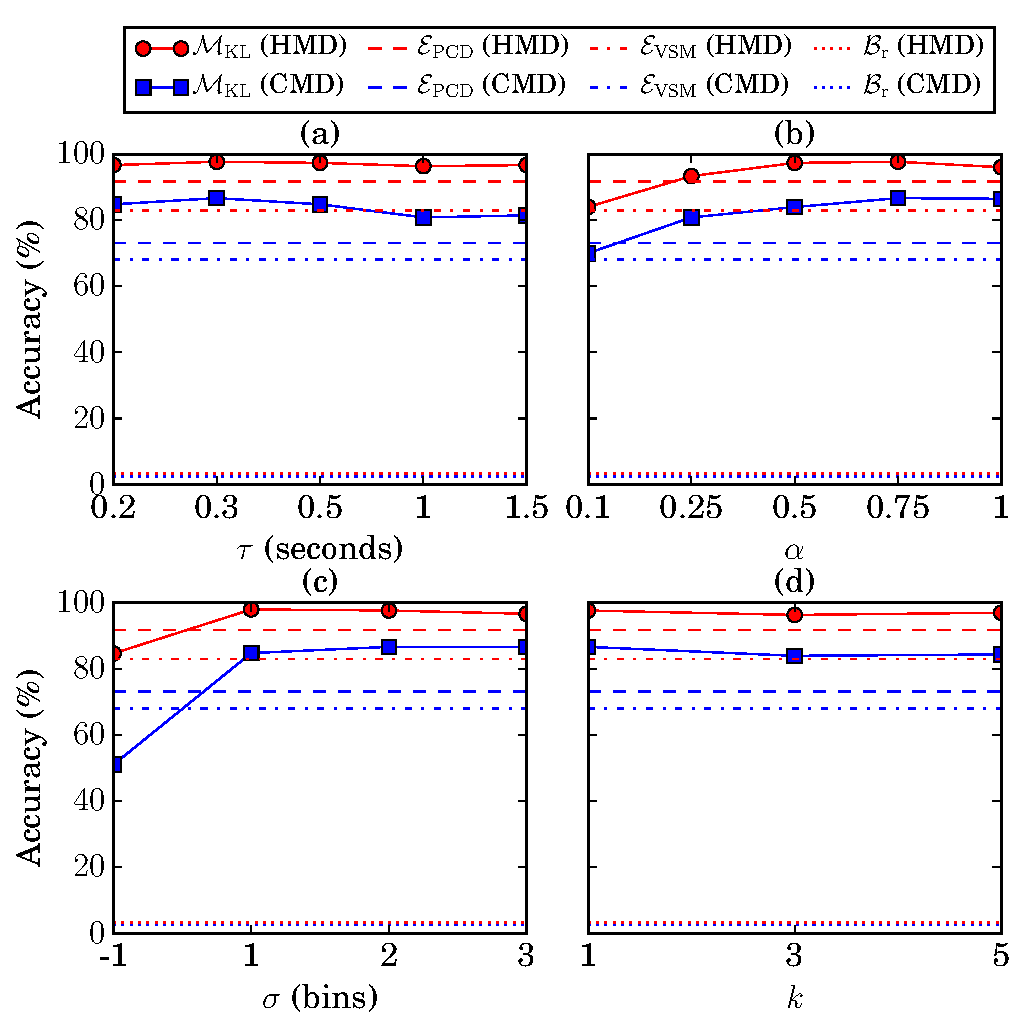
\includegraphics[width=\figSizeEighty]{ch07_ragaRecognition/figures/accuracy_vs_parameters_long2.pdf}
	\end{center}\vspace{-1em}
	\caption{Accuracy of \acrshort{ragarecTDMS_KL} as a function of parameter values. State-of-the-art approaches $\mathcal{E}$ and random baselines $\mathcal{B}$ are also reported for comparison.} 
	\label{fig:accuracy_vs_parameter_values}
\end{figure}

In Figure~\ref{fig:accuracy_vs_parameter_values}\,(a), we observe that the performance of the method is quite invariant to the choice of $\timeDelay$, except for the extreme delay values of 1 and 1.5\,s for CMD. This can be attributed to the melodic characteristics of Carnatic music, which presents a higher degree of oscillatory melody movements and shorter stationary svara regions, as compared to Hindustani music. In Figure~\ref{fig:accuracy_vs_parameter_values}\,(b), we see that compression with $\tdmsPowFac < 1$ slightly improves the performance of the method for both data sets. However, the performance degrades for $\tdmsPowFac < 0.75$ for  CMD and $\tdmsPowFac < 0.25$ for  HMD. This again appears to be correlated with the long steady nature of the svaras in Hindustani music melodies. Because the dynamic range of $\tdmsBase$ is high, \gls{tdms}\ features require a lower value for the compression factor $\tdmsPowFac$ to accentuate the surface values corresponding to the transitory regions in the melodies of Hindustani music. In Figure~\ref{fig:accuracy_vs_parameter_values}\,(c), we observe that Gaussian smoothing significantly improves the performance of the method, and that such performance is invariant across the chosen values of $\sigma$. Finally, in Figure~\ref{fig:accuracy_vs_parameter_values}\,(d), we notice that the accuracy decreases with increasing $k$. This is also expected due to the relatively small number of samples per class in our data sets~\cite{Mitchell97BOOK}. %The best accuracy obtained is for $k=1$, which is also reported in a previous study that uses PCD-based feature for the same task~\cite{chordia2013joint}. 
Overall, the method appears to be invariant to different parameter values to a large extent, which implies that it is easier to extend and tune it to other data sets.

\begin{figure}
	\begin{center}
		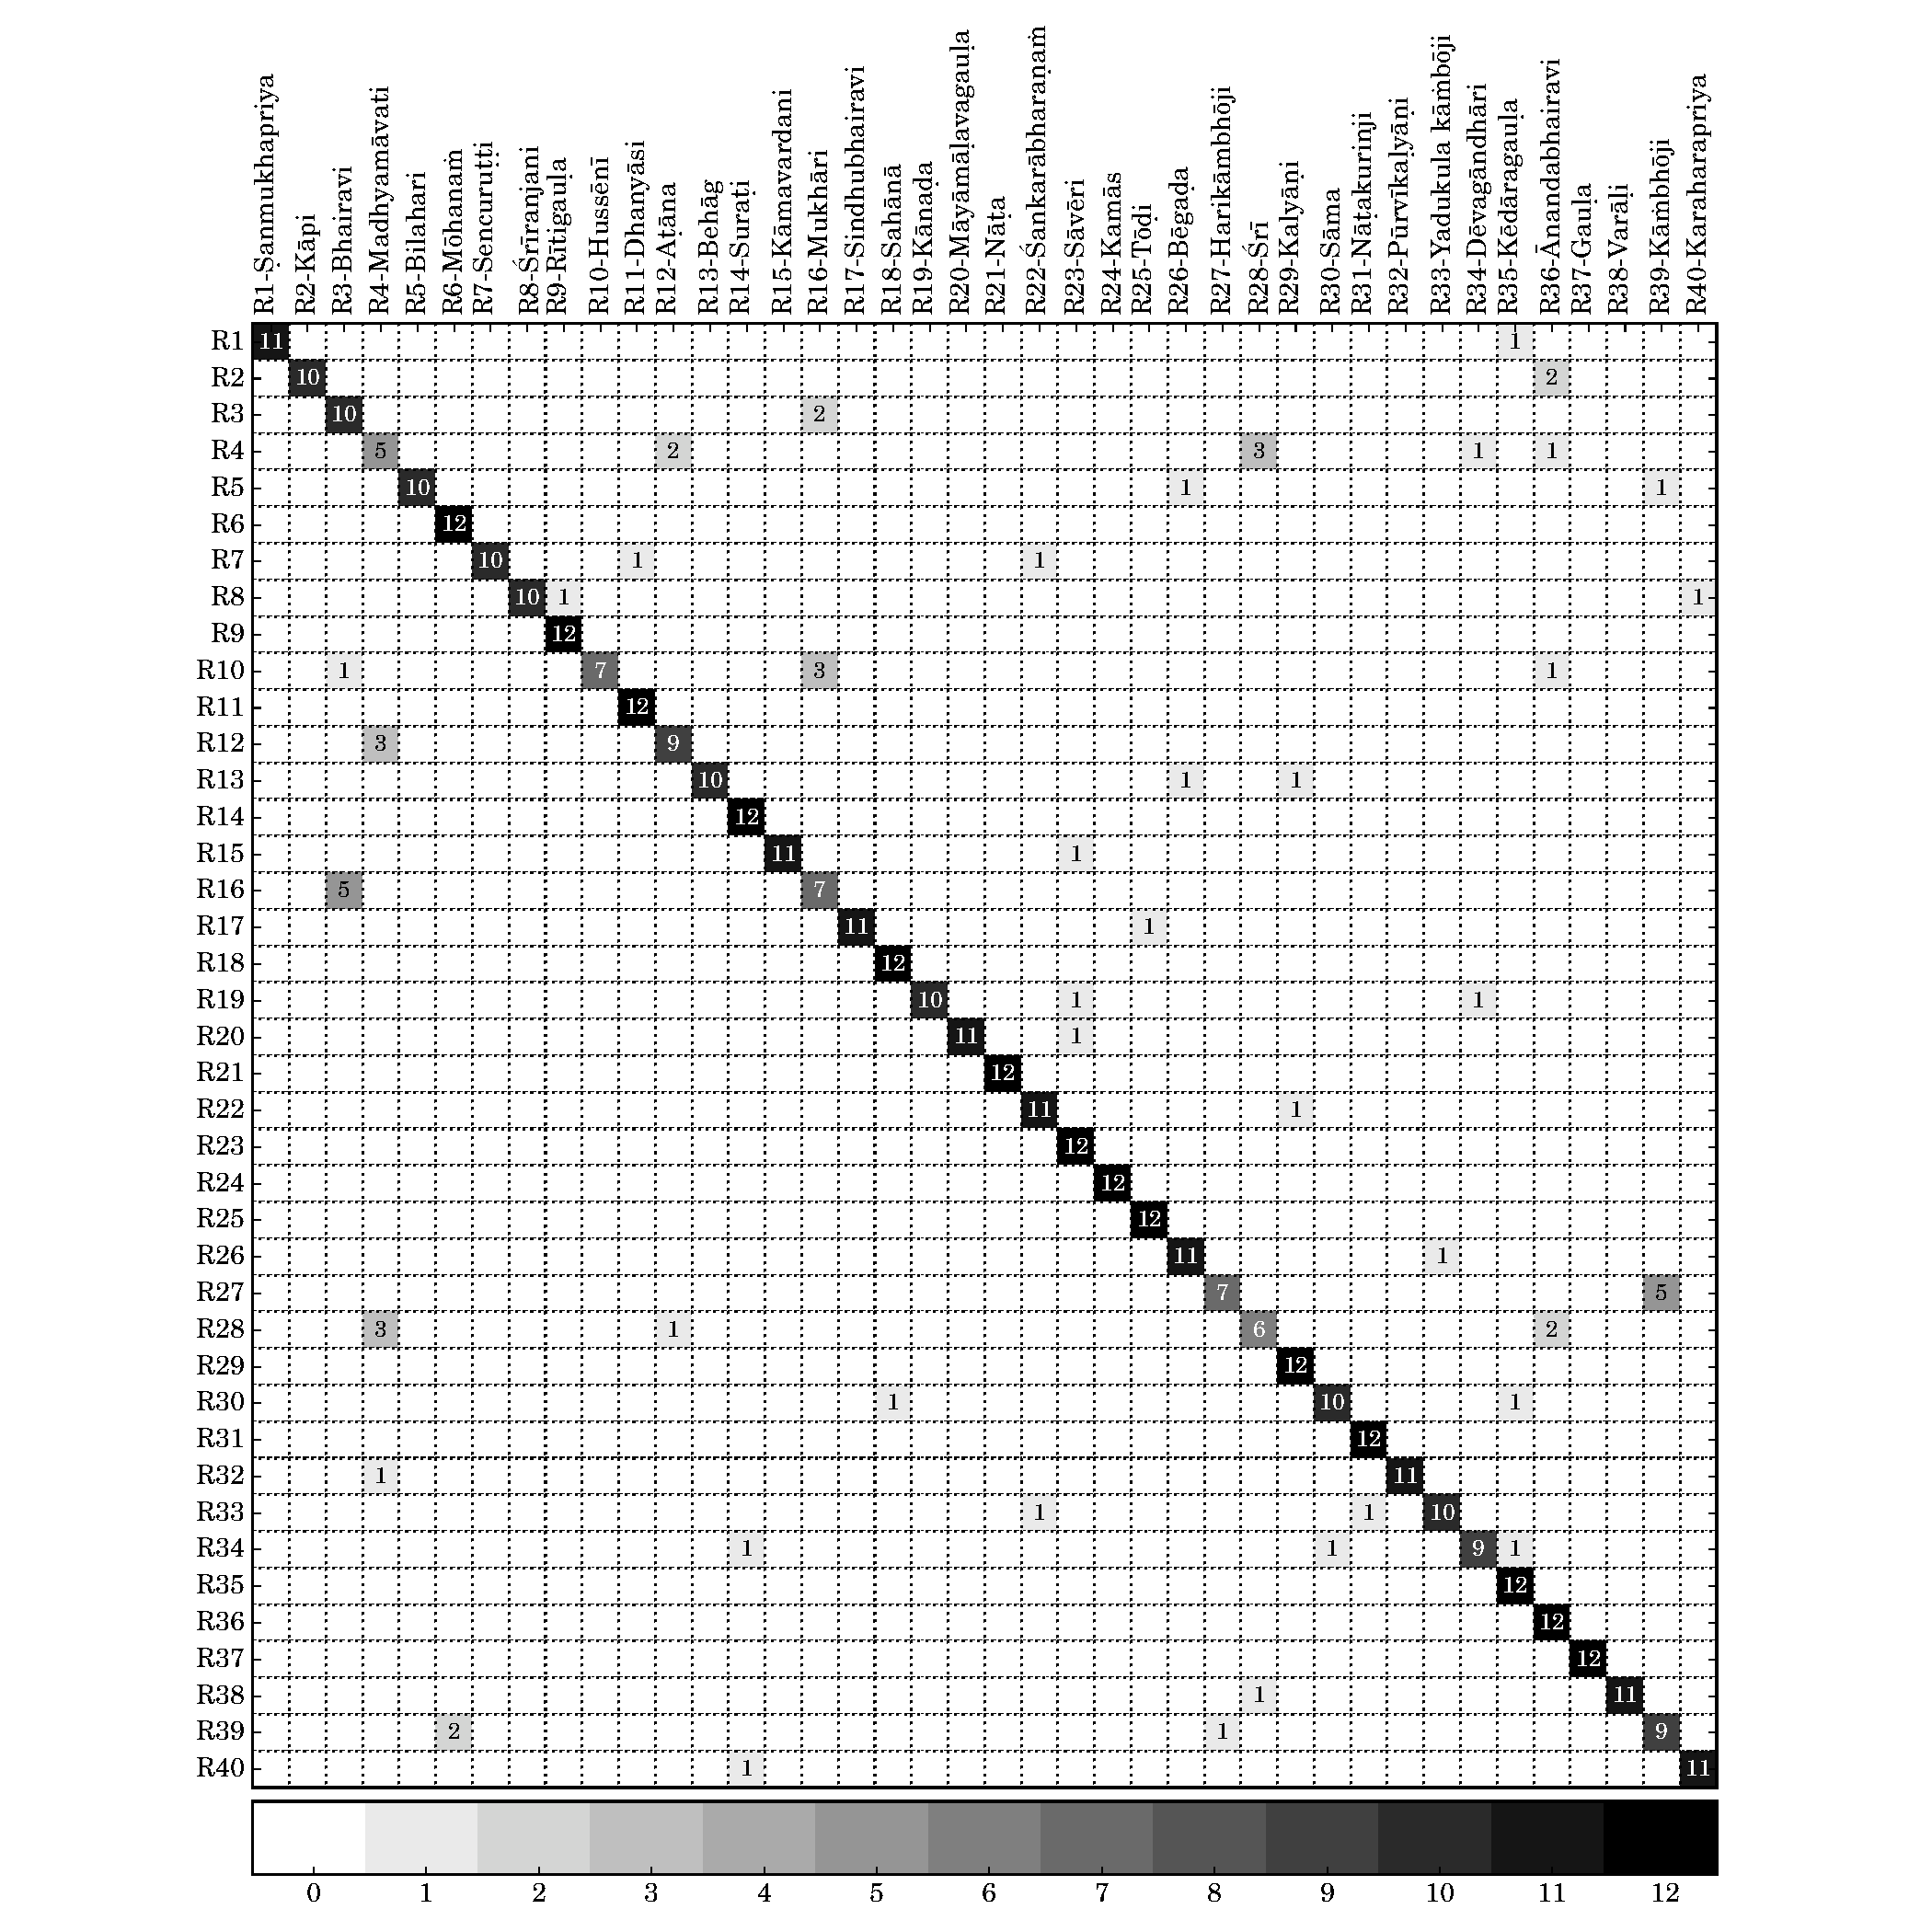
\includegraphics[width=\figSizeHundred]{ch07_ragaRecognition/figures/carnaticPhaseSapce_config_1078.pdf}
	\end{center}\vspace{-1em}
	\caption{Confusion matrix of the predicted \gls{raga} labels obtained by \acrshort{ragarecTDMS_KL} on CMD. Shades of grey are mapped to the number of audio recordings.} 
	\label{fig:confusion_mtx_carnatic}\vspace{-1em}
\end{figure}

From the results reported in Figure~\ref{fig:accuracy_vs_parameter_values}, we see that there exist a number of parameter combinations that could potentially yield a better accuracy than the one reported in Table~\ref{tab:main_results}. For instance, using  $\timeDelay=0.3$\,s, $\tdmsPowFac=0.5$, $\sigma=2$, and $k=1$, we are able to reach 97.0\% for \acrshort{ragarecTDMS_F} and 98.0\% for both \acrshort{ragarecTDMS_KL} and \acrshort{ragarecTDMS_B} on HMD. These accuracies are ad-hoc, optimizing the parameters on the testing set. However, and doing things more properly, we could learn the optimal parameters in training, through a standard grid search, cross-validated procedure over the training set~\cite{Mitchell97BOOK}. As our primary goal here is not to obtain the best possible results, but to show the usefulness and superiority of \gls{tdms} s, we do not perform such an exhaustive parameter tuning and leave it for future research.

%\begin{table} 
%	\centering
%	\resizebox{\linewidth}{!}{
%	\begin{tabular}{ c | c c c | c c}
%		\hline\hline
%		Data set   	& 	\acrshort{ragarecTDMS_F} 	&	\acrshort{ragarecTDMS_KL}		&	\acrshort{ragarecTDMS_B}	&	\acrshort{sotaChordia}		&	\acrshort{ragarecVSM}\\	
%		\hline
%		HMD   	& 	97.0 	&	{\bf 98.0}		&	{\bf 98.0} 	&	91.7		&	83.0\\
%		CMD   	& 	86.3	&	{\bf 86.7}		&	{\bf 86.7}	&	73.1		&	69.1\\
%		\hline\hline
%	\end{tabular}
%	}
%	\caption{Best in-sample accuracies (\%) of the three variants of the proposed method \acrshort{ragarecTDMS_F}, \acrshort{ragarecTDMS_KL} and \acrshort{ragarecTDMS_B}, and its comparison with the considered existing state-of-the-art methods \acrshort{sotaChordia} and \acrshort{ragarecVSM}.}
%	\label{tab:main_results_overfit}
%\end{table}


To conclude, we proceed to analyze the errors made by the best performing variant \acrshort{ragarecTDMS_KL}. For  CMD, we show the confusion matrix of the predicted \gls{raga} labels in Figure~\ref{fig:confusion_mtx_carnatic}. In general, we see that the confusions have a musical explanation. The majority of them are between the \glspl{raga} in the sets $\lbrace$Bhairavi, Mukh\={a}ri$\rbrace$, $\lbrace$Harik\={a}mbh\={o}ji, K\={a}mbh\={o}ji$\rbrace$, $\lbrace$Madhyamvat\={i}, A\d{t}\={a}na, \'Sr\={i}$\rbrace$, and $\lbrace$K\={a}pi, \={A}nandabhairavi$\rbrace$. \Glspl{raga} within each of these sets are allied \glspl{raga}~\cite{Viswanathan2004}, i.e., they share a common set of svaras and similar phrases. For HMD, there are only 7 incorrectly classified recordings (confusion matrix omitted for space reasons). \Gls{raga} Alhaiy\={a} bil\={a}wal and \gls{raga} D\={e}\'{s} is confused with \gls{raga} Gau\d{d} Malh\={a}r, which is musically explicable as these \glspl{raga} share exactly the same set of svaras. \Gls{raga} R\={a}g\={e}\'{s}hr\={i} is confused with B\={a}g\={e}\'{s}hr\={i}, which differ in only one svara. In all these cases, the \glspl{raga} which are confused also have similar melodic phrases. For two specific cases of confusions, that of \gls{raga}  Kham\={a}j with B\={a}g\={e}\'{s}hr\={i}, and \gls{raga} Darb\={a}r\={i} with Bh\={u}p, we find that the error lies in the estimation of the tonic pitch.


\section{Effect of Dataset}
\label{}

\section{Conclusions}
\label{sec:conclusions_raga_recognition}




